\subsubsection{Caso Particular GeM}
\label{subsec:exp8}
\begin{LaTeXdescription}
    \item[Objetivo] Analizar cuan ``justo'' es GeM, para un caso particular en
        el cual no haya dudas sobre lo que es justo y lo que no\footnote{O que
        haya muy poca probabilidad de que haya dudas al respecto.}.\\

    \item[Proposici\'on] Nos interesa analizar cu\'an ''justo'' es GeM para
        cierta definici\'on de justicia. Consideremos el caso de un torneo en
        que el equipo A le gana a todos los equipos salvo a B, y B pierde todos
        los partidos salvo el que le gana a A. Bajo nuestra definición de
        ''justicia'' o ''equidad'', o un aspecto de ella, A deber\'ia estar
        seguro por encima de B y B no deber\'ia estar por encima de muchos
        equipos (ya que perdi\'o contra todos). Observamos que en el caso del
        f\'utbol y su ránking 3-1-0 (o el esquema antiguo, 2-1-0) efectivamente
        B estar\'ia en la \'ultima posici\'on y A estar\'ia en la primera
        (eventualmente compartiendo dichas posiciones con alg\'un otro equipo).
        Entendemos entonces que este caso particular el ranking 3-1-0 es
        ''justo'' en este aspecto. Pero intu\'imos que esto no ser\'a lo que
        ocurra con GeM, ya que en el grafo de la instancia, A tiene un \'unico
        eje saliente (hacia B) y 18 entrantes, con lo cual su arista deber\'ia
        hacer subir mucho a B en el ranking.\\

    \item[Hip\'otesis] PageRank/GeM no es ''justo'' en cuanto al aspecto
        mencionado.\\

    \item[M\'etodo de Experimentaci\'on] Generamos una instancia de 20 equipos
        todos contra todos, donde existen A y B como se describieron. Entre los
        dem\'as equipos hacemos que el ganador sea aleatorios (con semilla =
        5). Todos los partidos terminan 1 a 0. Ejecutamos GeM y observamos el
        ranking final para diferentes valores de $\alpha$ (el factor de
        navegaci\'on).\\

    \item[Resultados, an\'alisis y discusi\'on]
\end{LaTeXdescription}

\begin{wrapfigure}{l}{0.5\textwidth}
    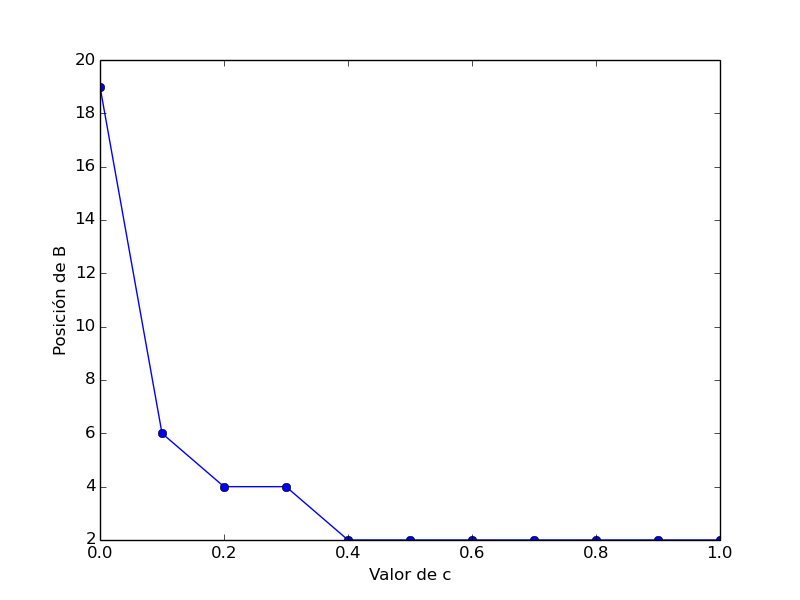
\includegraphics[width=0.5\textwidth]{exp8_posicion_B.png}
    \caption{Posici\'on del equipo B en el ranking en funci\'on del factor
        $\alpha$ ($c=\alpha$)}
    \label{fig:exp8_posB}
\end{wrapfigure}
\noindent

\par Lo primero que observamos es que B no ascendió al primer lugar para ningún
valor de $\alpha$, lo cual era esperable dados los resultados del experimento
\ref{subsec:exp7}, pero no deja de darnos cierta ``tranquilidad''. Sin embargo,
y como se puede ver en la figura \ref{fig:exp8_posB}, la posición del equipo B
sí mejora significativamente ya para valores pequeños de $\alpha$: un $\alpha =
0.1$ deja a B 6to en el ranking, y a partir de $\alpha = 0.4$ pasa a estar 2do.
Consideramos entonces que se confirmó nuestra hipótesis en el sentido de que GeM
no es ``justo'' en un caso del estilo. Como ya postulamos en el experimento
\ref{subsec:exp7}, no parece ``justo'' que un equipo prácticamente invicto que
tuvo un ``mal día'' le permita a otro equipo salir 2do en una competencia en la
que perdió con cuanto rival se cruzó.

\par Y no s\'olo eso. Supongamos ahora que el equipo A entra en una mala racha
y pierde muchos partidos consecutivos. Esto impactar\'a negativamente (para los
primeros partidos que pierda A luego de ser derrotado por B) en la ubicaci\'on
en el ranking de B. Es decir, B se ver\'a propulsado hacia las posiciones
superiores del ranking, pero luego comenzar\'a a perder posiciones no por
''m\'erito'' pr\'opio, sino por errores ajenos.

\par Podemos concluir entonces que los valores más ``justos'' de $\alpha$, para
evitar esta inestabilidad, serían los más bajos, dado que le dan menos
importancia a estas situaciones extrañas pero perfectamente posibles en
cualquier deporte.

\par Lo que observamos es que GeM a la hora de otorgar un puntaje, se fija
constantemente cual es el nuevo puntaje de aquellos equipos que hacen variar el
ranking de un equipo X, lo cual en un caso est\'atico no pareciera estar mal,
pero si lo pensamos en el tiempo avanzando fecha a fecha, podr\'ia ser injusto a
los ojos de alguno\footnote{Ni hablar de las posibilidades de fraude. ''Vos me
ganaste, y si ahora yo salgo a perder te perjudico''. \emph{Imagine the
possibilites}.}. Ejemplifiquemos esto \'ultimo: supongamos que Racing, en zona
de descenso, le gana al puntero del campeonato y a partir de la inestabilidad
encontrada en GeM, pasa a estar fuera de la zona de descenso. Pero ahora depende
de que el puntero siga ganando, sino quiere volver a dicha zona. La mayor\'ia de
los rankings oficiales de los deportes evitan esto, ya que equiparan los puntos
que se reciben por ganarle a cualquier equipo (no hay diferencia en cuanto a
ganarle al puntero que a un equipo de media tabla).

\par Para finalizar, diremos que si bien se encontr\'o esta inestabilidad en el
modelo GeM, si esto es perjudicial o no depender\'a del contexto de uso. La
utilizaci\'on de este esquema para determinar el orden de los competidores en
alg\'un evento deportivo podr\'ia dar lugar a situaci\'ones mejores o peores.
Como siempre, con esto y con casi todas las cosas, su aplicaci\'on, beneficios y
desventajes dependeran del contexto de uso.
